\vspace{-2pt}
\subsection{MAAR Platform Evaluation in DSE}
\label{subsec:res-overall}

To understand the benefits of MAAR Evaluation, this section compares MAAR DSE with DSS~\cite{zhang2018ds} and 1appDSE. DSS is a greedy algorithm for many-application platform allocation according to characteristics analysis across applications without an evaluation. 1appDSE considers one application in isolation instead of many applications. In the experiments, an exhaustive search is used to find the 1appDSE platform, which gives the optiamal (OPT) platform for one application. Then mapping all applications on this platform provides one 1appDSE platform performance. To get the average performance of 1appDSE, this paper maps all applications onto all OPT platforms (one platform from one application). Similar to OOP, 1appDSE results in the same number of platforms. However, OOP only maps the application on its Own Optimal Platform, while 1appDSE maps all applications onto each platform.

%In this experiment, 1appDSE and OOP have the same set of platforms. However, OOP only maps the application on its Own Optimal Platform, while 1appDSE maps all applications onto each platform.
%

\begin{figure}[h]
\vspace{-8pt}
	\centering
		\subfloat[Average $rEFF_{SW}$] {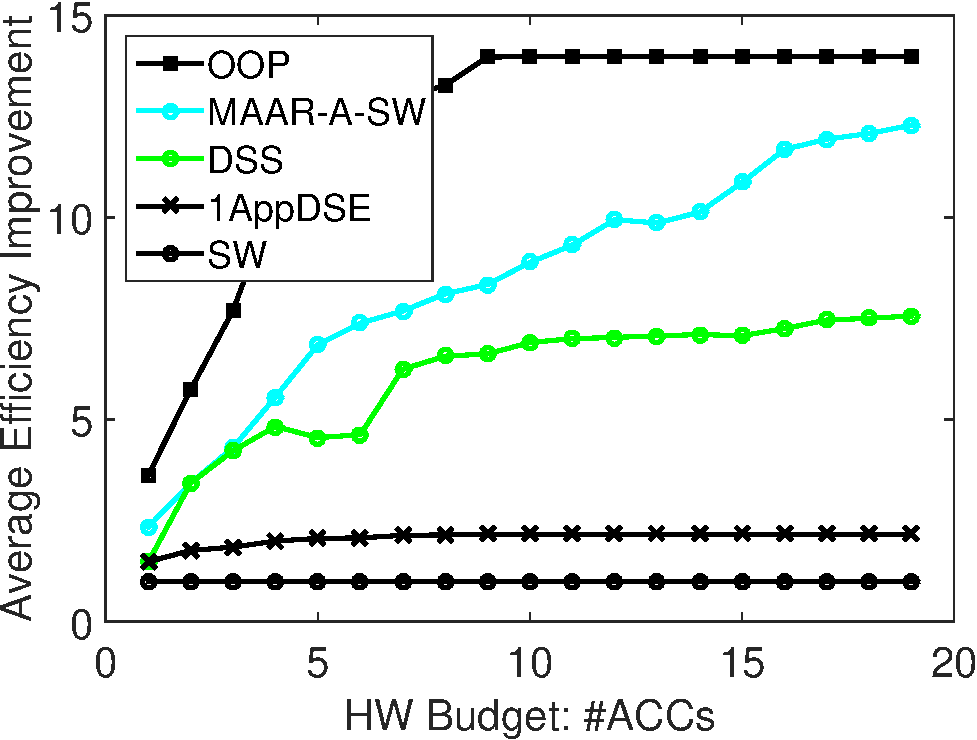
\includegraphics[width=.33\linewidth]{fig/allsw.pdf}\label{fig:allsw}}
		\hfill
		\subfloat[Average $rEFF_{OOP}$] {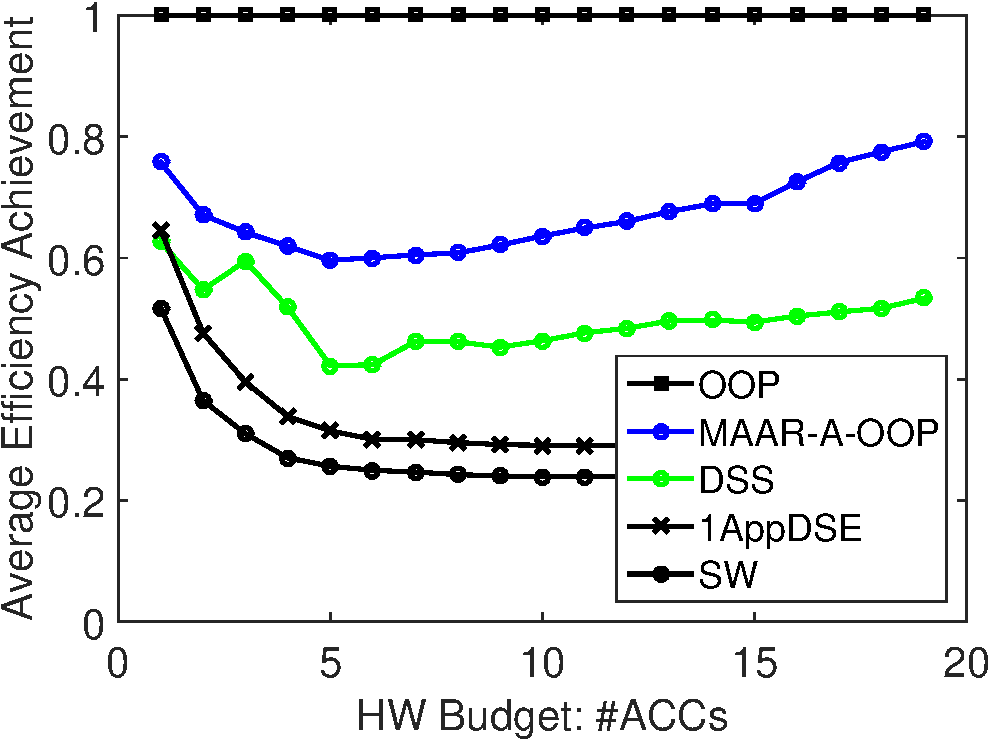
\includegraphics[width=.33\linewidth]{fig/alloop.pdf}\label{fig:alloop}}
		\hfill
		\subfloat[Unique ACCs Used] {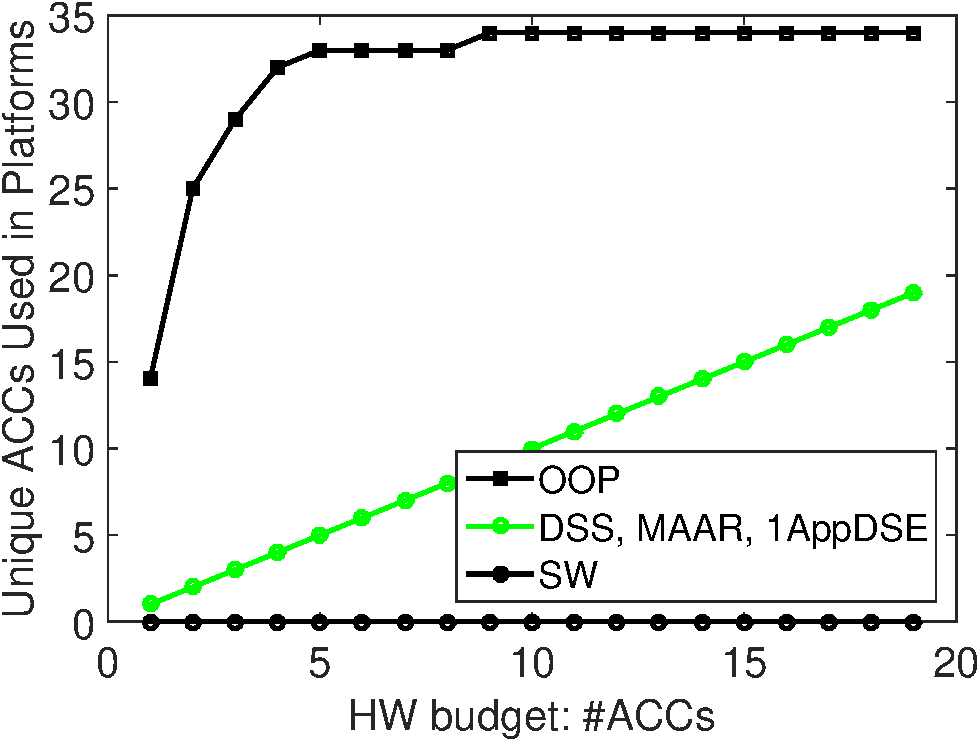
\includegraphics[width=.33\linewidth]{fig/oopHW.pdf}\label{fig:oopHW}}
	\vspace{-8pt}
	\caption{OpenVX: DSE Methods Comparison }
	\label{fig:avg}
\end{figure}

\figref{fig:allsw} shows the average efficiency improvement ($rEEF_{SW}$) across all applications of different DSE platforms over increasing ACCs budgets. OOP yields the absolute upper bound for a given HW constraints. OOP plateaus after ACCs=9, since each application only has up to 10 unique kernels. Since SW compared with itself, the $rEFF_{SW}$ value of SW is always equal to 1, which yields the lower bound. MAAR DSE uses $A\mhyphen SW$ (average aggregation of $rEEF_{SW}$) evaluation. MARR-A-SW's average efficiency improvement increases with the number of ACCs. It approaches the OOP efficiency when ACCs=19. On average across the HW budgets, MAAR has 1.39 times the efficiency improvement of DSS, and 4.01 times the improvement of 1AppDSE.

\figref{fig:alloop} shows the average efficiency achievement ($rEEF_{OOP}$) across all applications of different DSEs. OOP always achieves 100\% efficiency compared to itself, and is the upper bound. SW has the lowest efficiency achievement, only reaching about 24\% after ACCs>9. MAAR DSE uses $A\mhyphen OOP$ (average aggregation of $rEFF_{OOP}$) evaluation and produces a much better efficiency achievement than other DSEs. On average across the HW budgets, MAAR has 1.35 times the efficiency achievement of DSS, and 2.12 times the achievement of 1AppDSE. \figref{fig:alloop}, also shows MAAR has a lower improvement speed than OOP when the HW budget is less than 5. However, after this point, MAAR improves faster than OOP. As OOP has already accelerated almost all computationally expensive kernels, there are less potential efficiency improvement for OOP.  

%Since efficiency achievement is relative to OOP, the plot of DSE can also describe the improvement speed between the DSE and OOP.
%MAAR is decreasing while ACCs<5, and increasing while ACCs>5. This 

\figref{fig:oopHW} lists the number of unique ACCs for each DSE (SW is empty; DSS, MAAR and 1AppDSE are equal to the budget). OOP has one platform per application, so there are 40 platforms for all applications. Each OPT platform has a number of HWACCs equal to the budget, so there are a large number of unique ACCs. When each OPT platform has 1 ACC, there are 14 unique ACCs, indicating some reuse. However, if each OPT platform has 2 ACCs, there are 25 unique ACCs (11 more) showing the limits of reuse. This also shows limits of composability of single App DSE. In \figref{fig:alloop}, the MAAR with a 2 HWACCs budget allocates \emph{Custom Convlution} and \emph{Canny Edge Detector} kernels, and achieves 67\% the average energy efficiency of OOP, which uses 25 unique ACCs in OOP. This shows a MAAR accelerating a small number of high-computing kernels can achieve good energy efficiency across many applications.

% the order of kernel in OpenVX allocation. CustomConvolution CannyEdgeDetector HarrisCorners OpticalFlowPyramid(LK)  BoxFilter GaussianFilter